\chapter{Founding Experiments and Notions of Particle Accelerators and Detectors}

%%%%%%%%%%%%%%%%%%%%% chapter.tex %%%%%%%%%%%%%%%%%%%%%%%%%%%%%%%%%
%
% sample chapter
%
% Use this file as a template for your own input.
%
%%%%%%%%%%%%%%%%%%%%%%%% Springer-Verlag %%%%%%%%%%%%%%%%%%%%%%%%%%
%\motto{Use the template \emph{chapter.tex} to style the various elements of your chapter content.}
%\chapter{Particle accelerators and colliders}
\label{accelerators} % Always give a unique label
% use \chaptermark{}
% to alter or adjust the chapter heading in the running head
\section{Particle accelerators}
We have seen the importance of probing nuclei and particles at high energy. One clear example is given by the weak interactions, where new phenomena (propagator of the interaction) are expected at an energy of the order of $10^5$ MeV. In order to reach high energies, at the beginning  cosmic rays and radioactive sources were used; later on, people started building particle accelerators.

Particle accelerators are extremely complex machines which are based on fundamental, but simple, principles. Those are:
\begin{itemize}
  \item source of particles to be accelerated;
  \item accelerating elements (with electric field);
  \item magnetic elements to bend or focus the beams of particles.
\end{itemize}

\subsection{Electrostatic accelerators}
The simplest particle accelerator is the cathodic tube of Thomson, described in Chapter \ref{Fundamentals-I}. A static electric field, however, is limited by discharging effects. 

The two main static accelerators are:
\begin{enumerate}
    \item \label{item2:Cockroft-Walton} the Cockcroft-Walton accelerator;
    \item \label{item2:Van der Graaf} the Van der Graaf accelerator.
\end{enumerate}

The Cockcroft-Walton accelerator, schematized in Figure \ref{fig:Cockcroft-Walton}, is able to raise a low  alternate current to an high direct voltage trough a system of diodes and capacitors, placed in a tower structure in order to \textit{raise} and \textit{level} the voltage. It is possible to obtain voltages of the order of \SI{1}{MV} and consequently they can be used to accelerate particles to energies of about \SI{1}{MeV}.

\begin{figure}
    \centering
    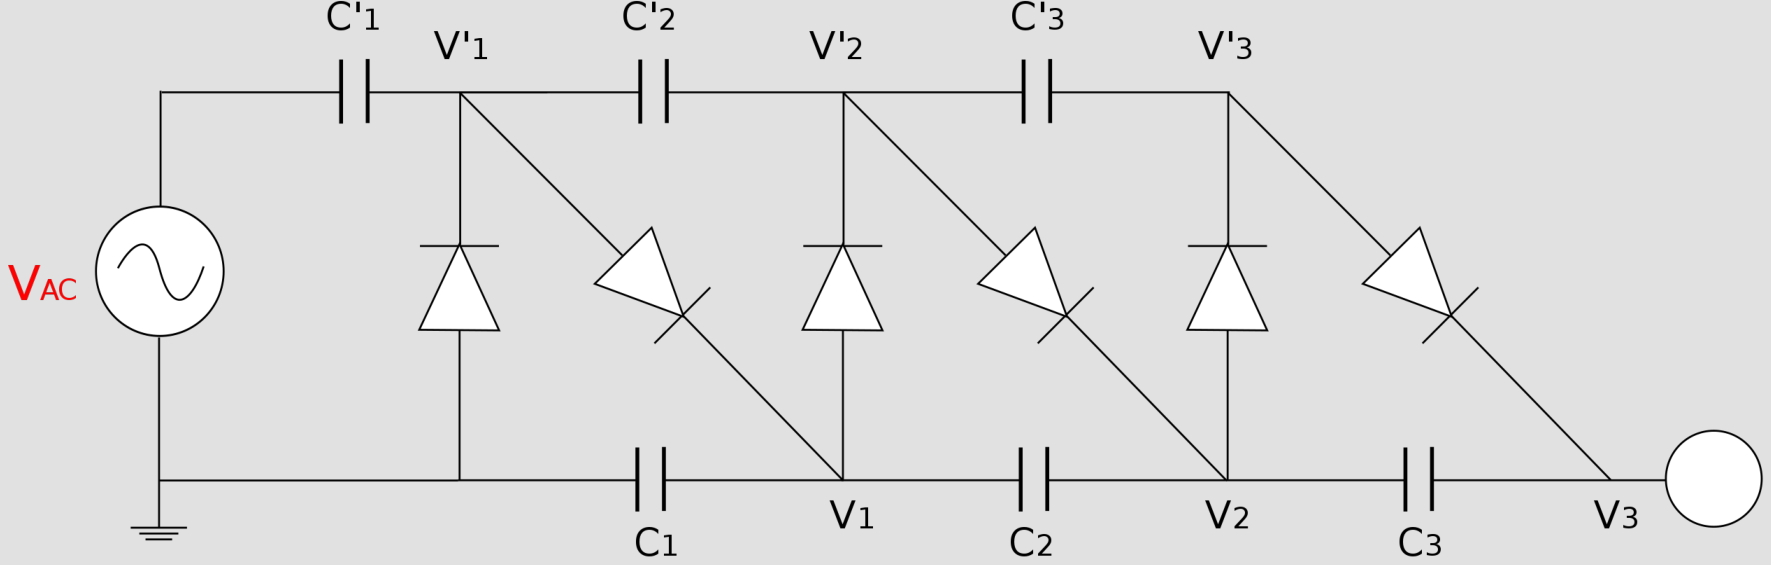
\includegraphics[width=0.8\textwidth]{Figures/Cockcroft-Walton}
    \caption{Schematic view of a Cockcroft-Walton machine. The primed capacitors ($C'$) are the one used to increase the voltage while the other ones are used to level the output of the machine.}
    \label{fig:Cockcroft-Walton}
\end{figure}

The second type of accelerator is the Van der Graaf accelerator. As for the Cockroft-Walton accelerator, this has been developed between 1929 and 1930. Represented in Figure \ref{fig:Van-der-Graaf}, the Van der Graaf accelerator is an electrostatic machine featuring a transport belt (made of insulating cloth) which is used to move the electric charges. The belt, moved by an engine, accumulates the charges onto a conductive sphere which is located in a elevated position in order to isolate the charges from the ground.

In this way it is possible to reach voltages of the order of a few \si{MV}. The highest value ever reached with this kind of machine is \SI{25}{MV}. To go to higher energies new techniques are needed, like for example having particless pass more times through the accelerating fields.

\begin{figure}
    \centering
    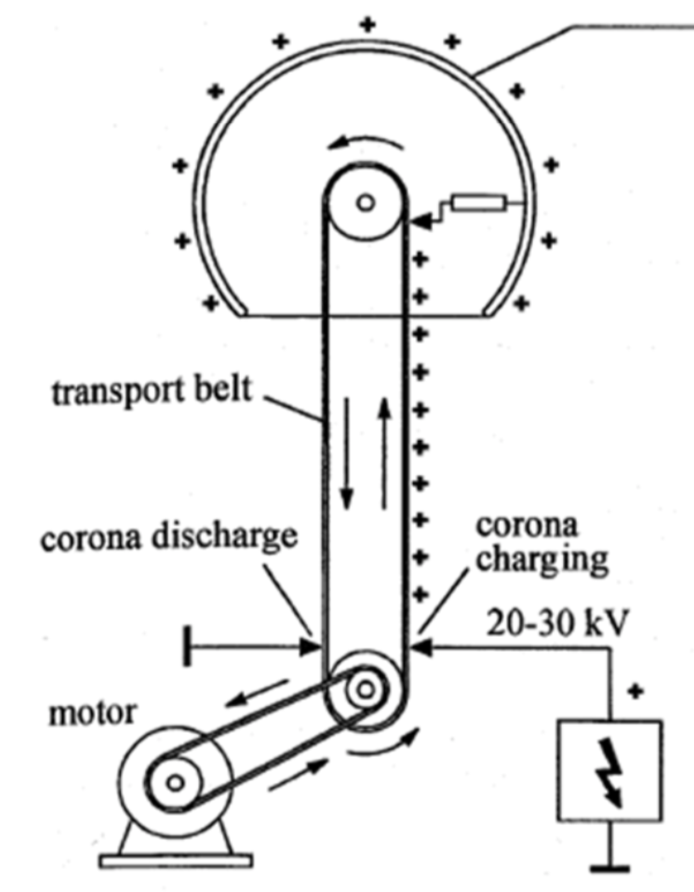
\includegraphics[width=0.3\textwidth]{Figures/Van-der-Graaf}
    \caption{Schematic view of a Van der Graaf generator.}
    \label{fig:Van-der-Graaf}
\end{figure}

\subsection{Wideroe's linear accelerator}
The first linear accelerator featuring an alternated electric field was built by Wideroe (1928) and is represented in Figure \ref{fig:Wideroe-linear-accelerator}. 
\begin{figure}
    \centering
    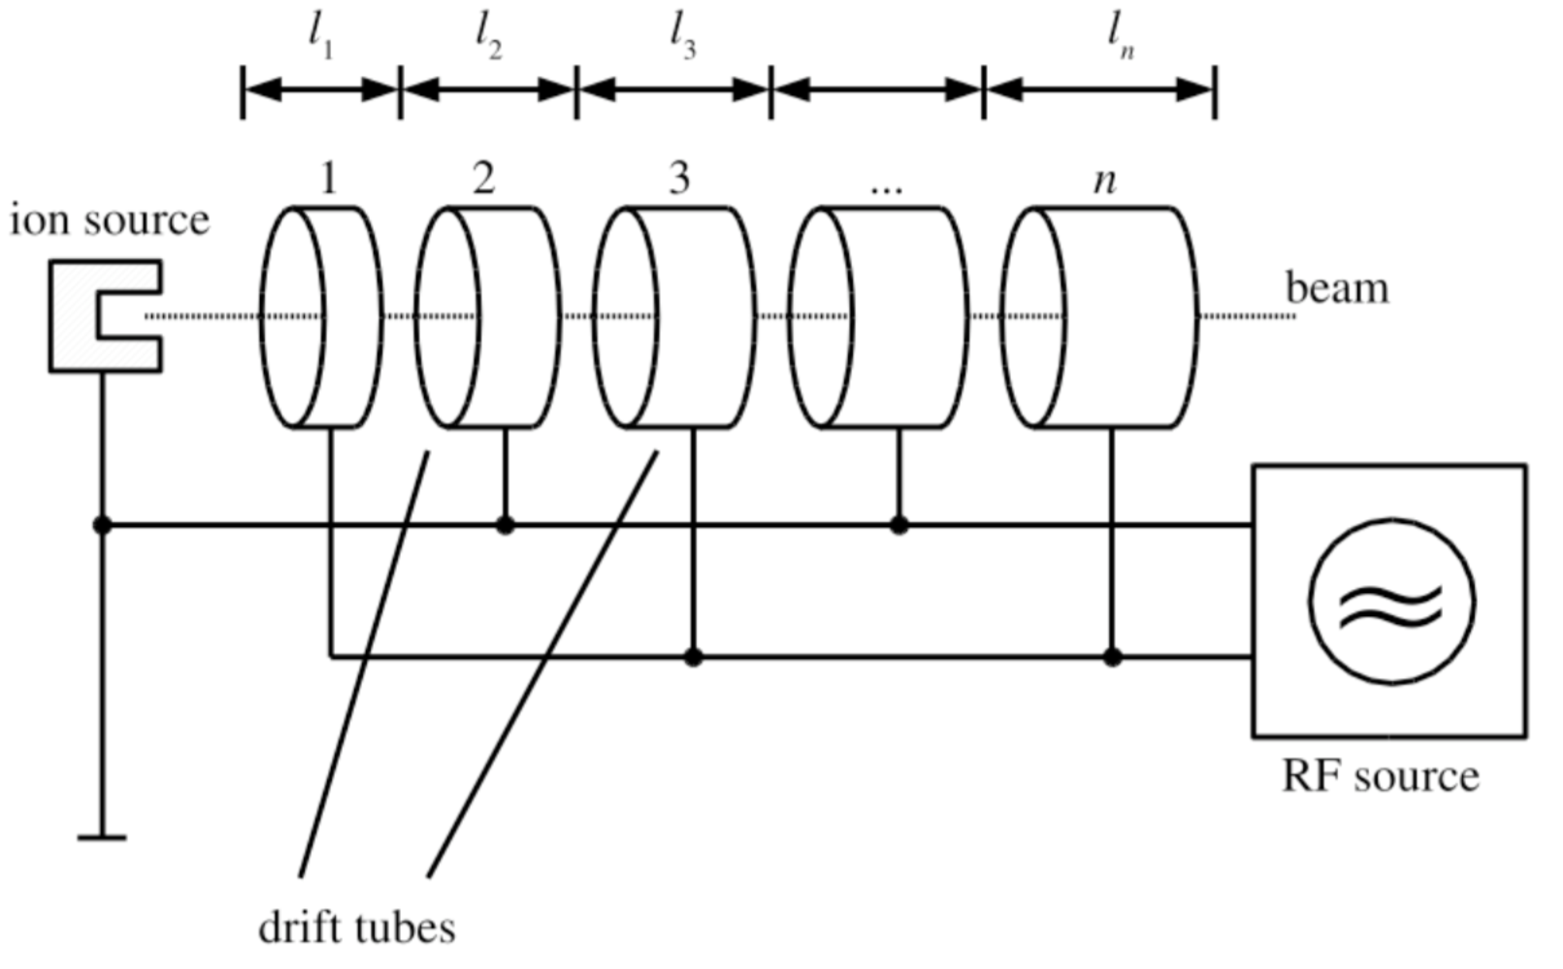
\includegraphics[width=0.6\textwidth]{Figures/Wideroes-linear-accelerator}
    \caption{Schematic of the Wideroe's linear accelerator}
    \label{fig:Wideroe-linear-accelerator}
\end{figure}
In order to accelerate the particles without using high voltages, it is possible to use oscillating voltages built in a way that in each passage the field is in phase with the particles to be accelerated. The path of the particles is fragmented into a series of metallic pipes which act as Faraday's cages. The poles from a single generator are connected in order to invert the voltage of the accelerating fields in the time interval in which the particles goes through the pipe. Increasing lengths of the Faraday's cages, $l_{\small{\text{i}}}$, are chosen, in order to maintain constant the time needed to go trough them, which is the inverse of the frequency of the generator, $t = 1 / f_{RF}$.

\subsection{Cyclotrons}
Another way to achieve multiple passages through an oscillating electric field is adopted in cyclotrons. These machines are circular accelerators in which the frequency of the oscillating field is by construction constant, while the path of particles is controlled by a fixed magnetic field.

The functional principle is obtained equating the Lorentz force to the centripetal acceleration,
\begin{equation}
    qvB = \frac{mv^2}{r},
    \label{eq:cyclotrons}
\end{equation}
where $q$ is the electric charge of the particle, $v$ its velocity, $B$ the magnetic field, $m$ the mass and $r$ the curvature radius.
From Eq. \eqref{eq:cyclotrons}, one immediately obtains
\begin{equation*}
    mv = qBr,
\end{equation*}
so
\begin{equation*}
    r = \frac{mv}{qB}
\end{equation*}
is the curvature radius in a magnetic field. Keeping in mind that the angular velocity is $\omega = \frac{v}{r}$, the rotational frequency is obtained as
\begin{equation*}
    f_{c} = \frac{\omega}{2\pi} = \frac{v}{2\pi r} = \frac{qB}{2\pi m},
\end{equation*}
and does not depend on the radius of the trajectory. As a consequence, it is enough to fix an alternate voltage to obtain, by construction, a synchronisation.

This principle is valid until particles reach the relativistic regime. In this case a correction needs to be applied to the voltage frequency, which becomes
\begin{equation*}
    f = \frac{f_{c}}{\gamma}.
\end{equation*}
This means that the frequency is no more fixed, but must be adjusted during the accelerating procedure. To achieve this, two options are available:
\begin{itemize}
    \item adjust the cyclotron frequency while operating: Cyclo-synchrotrons;
    \item adjust the intensity of the magnetic field: Isosynchronos-cyclotrons - the magnetic field is increased as the radius increases.
\end{itemize}
The first concept of a \SI{9}{in} ($~\SI{23}{cm}$) cyclotron is represented in Fig. \ref{fig:Cyclotron}.
\begin{figure}
    \centering
    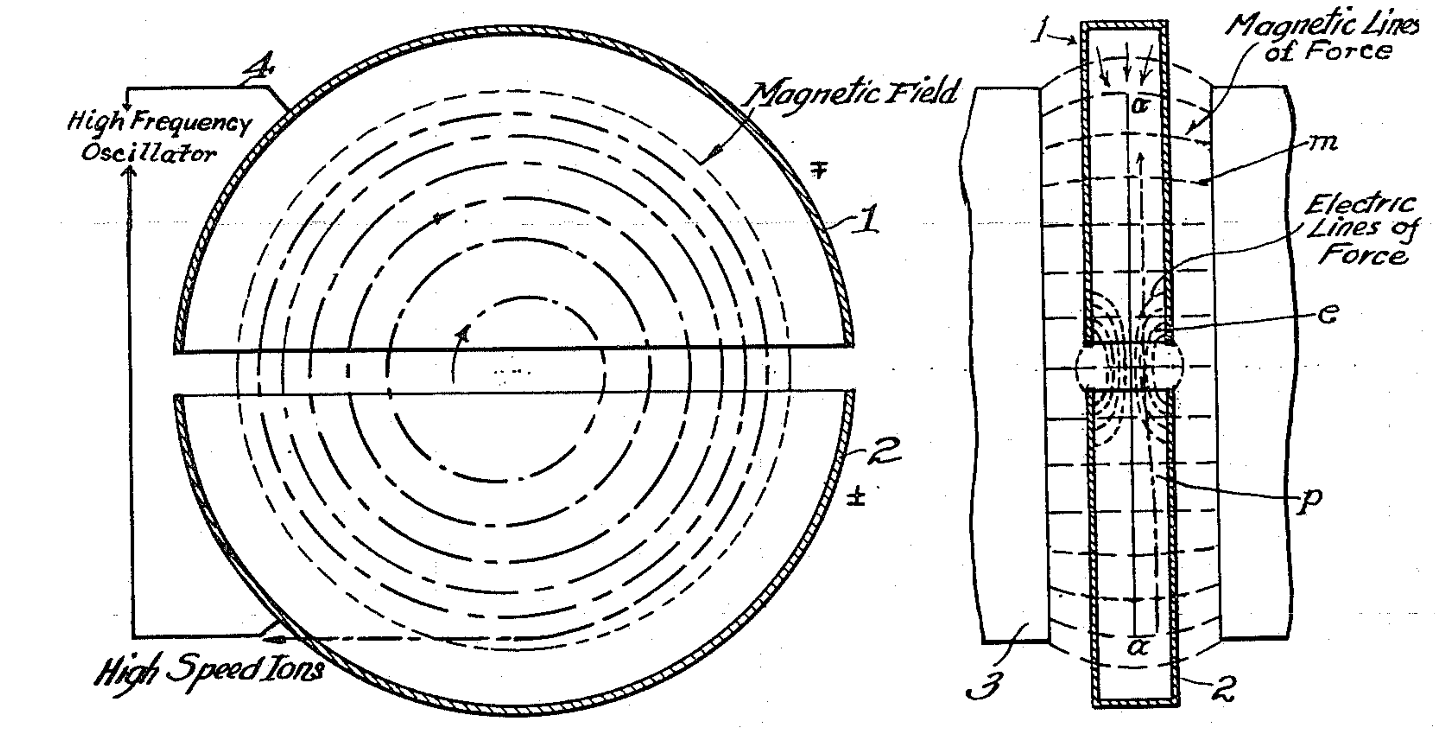
\includegraphics[width=0.8\textwidth]{Figures/Cyclotron}
    \caption{Cyclotron patent from 1931.}
    \label{fig:Cyclotron}
\end{figure}

With simple cyclotrons it was possible to accelerate particles up to \SI{100}{MeV}, while with cyclo-synchrotrons up to \SI{1}{GeV}.

\subsection{Synchrotrons}
The idea of the synchrotron is to have a fixed-radius orbit, in order to be able to build larger machines with the same principle of the linear accelerators: while the electric field is in a decelerating mode, the particles are screened by Faraday's cages. The longitudinal electric field is created by resonant cavities with radio frequencies that produce electromagnetic waves with a longitudinal component which could either accelerate or decelerate charged particles. Therefore, particles need to be synchronised with the machine.

Magnetic elements are used to bend particles in order to constrain them to circular paths. The bending power must increase with higher energies and frequency needs also to be increased in order to maintain synchronisation. An important aspect of the circular motion with fixed radius is that relativistic particles start to loose energy due to irradiation (bremsstrahlung). This plays a central role in setting the maximum achievable energy, and  is related to the kind of particle which is accelerated. In fact, the irradiated power of an accelerated charge with acceleration $a$ and charge $e$ can be expressed as
\begin{equation*}
    W = \frac{1}{6\pi\varepsilon_0c^3}e^2a^2,
\end{equation*}
and taking into account relativistic effects it becomes
\begin{equation*}
    W = \frac{1}{6\pi\varepsilon_0c^3}\gamma^6e^2\left(a^2-\frac{1}{c^2}(\Vec{v}\times\Vec{a})^2\right).
\end{equation*}
For a circular motion of radius $R$, the following relations hold:
\begin{equation*}
    \Vec{v}\times\Vec{a} = va \;\;\;\;\;\text{and}\;\;\;\;\; a = \frac{v^2}{R},
\end{equation*}
therefore the irradiated power can be expressed as 
\begin{equation*}
    W = \frac{e^2}{6\pi\varepsilon_0c^3}\frac{\gamma^4v^4}{R^2}.
\end{equation*}
Using the relation $E = \gamma mc^2$, for $v \rightarrow{c}$ one gets
\begin{equation}
    W = \frac{e^2c}{6\pi\varepsilon_0R^2}\frac{E^4}{(mc^2)^4}.
    \label{eq:irradiated-power}
\end{equation}
Equation \ref{eq:irradiated-power} shows that the irradiated power grows with the fourth power of the energy, and it is inversely proportional to the fourth power of the mass. The irradiated power of an electron is $10^{13}$ times greater than the one of a proton with the same energy.
This energy loss is commonly referred to as \emph{synchrotron radiation}.

For an electron synchrotron, the maximum reachable energy is therefore limited by the maximum acceleration reached in the radio-frequency cavities needed to compensate the energy loss due to irradiation. For a proton synchrotron, instead, the maximum energy is limited by the bending power of the magnets used in the machine, which are needed to maintain the circular orbit. A schematic view of the elements of a synchrotron is shown in Fig. \ref{fig:Synchrotron}, while a picture of the Cosmotron built in Brookhaven is shown in Fig. \ref{fig:Cosmotron}.

\begin{figure}[h]
    \centering
    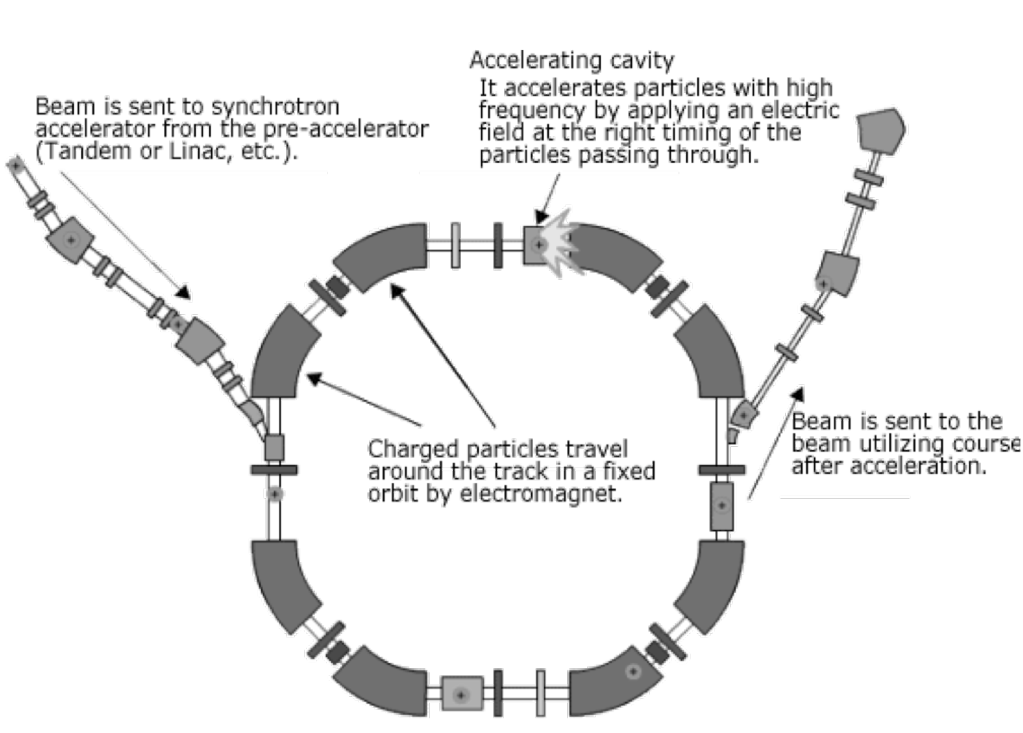
\includegraphics[width=0.75\textwidth]{Figures/Synchrotron}
    \caption{Schematic view of the elements of a synchrotron by V. Kain (CERN).}
    \label{fig:Synchrotron}
\end{figure}
\vspace{3.5cm}
\begin{figure}[h]
    \centering
    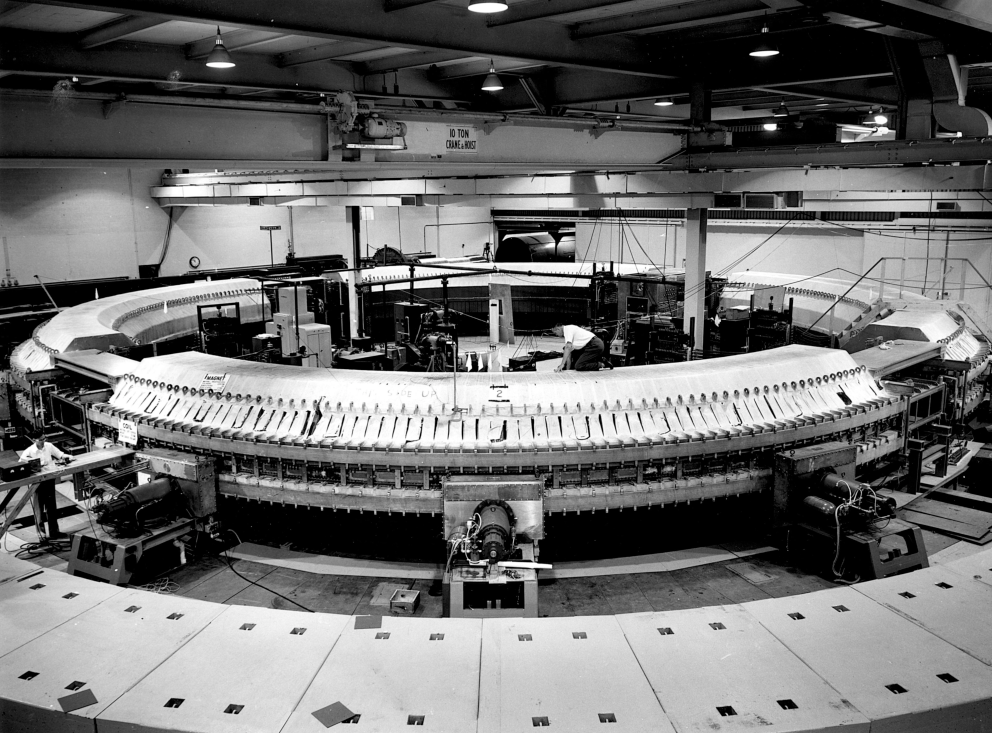
\includegraphics[width=0.65\textwidth]{Figures/Cosmotron}
    \caption{Picture of the Cosmotron, a proton synchrotron which operated at Brookhaven laboratories until 1968.}
    \label{fig:Cosmotron}
\end{figure}
 % particle accelerators

\section{Particle Detectors}
The main purpose of particle detectors is to detect particles and to measure their properties, such as:
\begin{itemize}
\item trajectory in space and time;
\item charge and momentum;
\item deposited energy when interacting with matter.
\end{itemize}
These three properties are well known and constitute a well-motivated way to discriminate between (``identify'') particles.

The detection process is strictly related to the way particles interact in the material of which the detector is composed. The energy of the particle is transferred to the medium and undergoes a process of \emph{conversion} into another form which can be detected.

\begin{figure}
  \centering 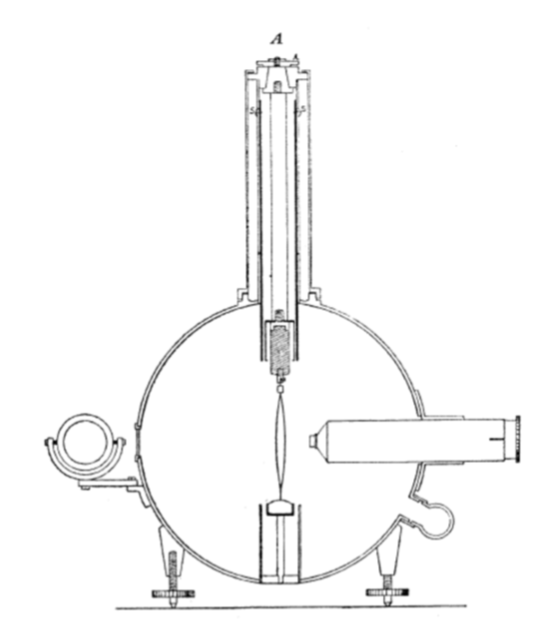
\includegraphics[width=0.5\textwidth]{detector1}
  \caption{Electrometer sensible to ionisation, developed by T. Wulf (1909).}
  \label{fig:detector1}
\end{figure}

\begin{figure}
  \centering 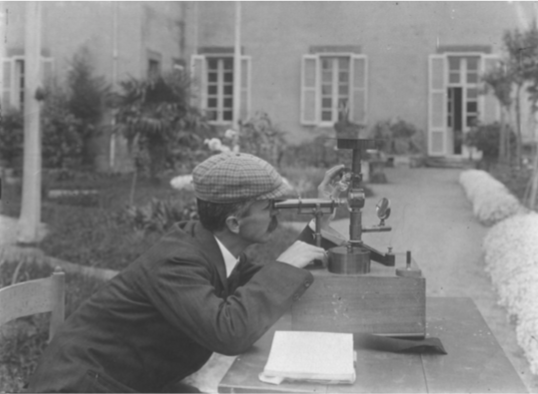
\includegraphics[width=0.5\textwidth]{detector2}
  \caption{Rome, 1910: using the Wulf electrometer, Pacini measured a significant rate variation of cosmic ray interactions with height, in particular under $3\,\meter$ of water.}
  \label{fig:detector2}
\end{figure}

\begin{figure}
  \centering 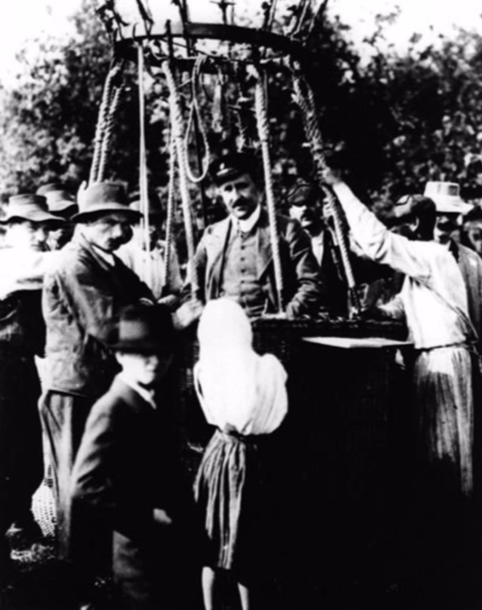
\includegraphics[width=0.5\textwidth]{detector3}
  \caption{1912: Hess installed an electrometer on a balloon and measured that the counting rate at $5300\,\meter$ was four times the observed rate at ground level. The hypothesis that this radiation originated from the Sun was excluded because the measure had been repeated during an eclipse.
  The radiation observed was due to \emph{cosmic rays}.}
  \label{fig:detector3}
\end{figure}

\subsection{Detectors of charged particles}\label{sec:detector1}
It is possible to identify, between the various processes which are today used in particle detectors, four main processes -- and, correspondingly, four different kinds of detectors:
\begin{itemize}
\item ionisation detectors;
\item scintillation detectors;
\item semiconductors;
\item Cherenkov detectors.
\end{itemize}

\subsubsection*{Ionisation detectors}
In a gaseous medium, ionisation corresponds to the creation of electron--ion (or electron--nucleus) pairs along the path of a particle which crosses its material. The minimum energy to create a pair is $\sim 20\div30\,\electronvolt$.

The ionisation can be measured in many different ways. One simple method consist in applying a very strong electric field to observe a discharge when a charged particle crosses the medium. This is the principle on which the \emph{Geiger--Muller counter} is based (1913).

\begin{figure}
  \centering 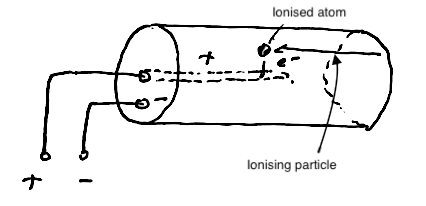
\includegraphics[width=0.5\textwidth]{detector5}
  \caption{After a charged particle has crossed the detector, a discharge is observed.}
  \label{fig:detector5}
\end{figure}

Electrons produced in the ionisation are immediately accelerated by the electric field, originating further (``secondary'') ionisations which start an avalanche process (\emph{Townsend avalanche}).

\begin{figure}
  \centering 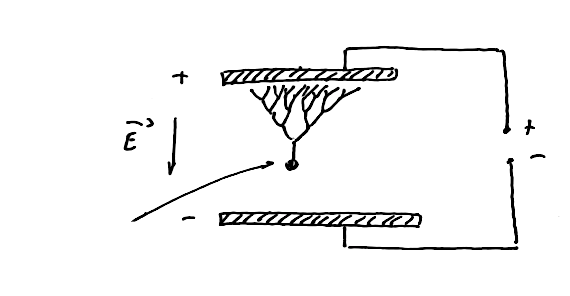
\includegraphics[width=0.5\textwidth]{detector4}
  \caption{Example of an avalanche process originated after the primary ionisation using an electric field $E$.}
  \label{fig:detector4}
\end{figure}

\subsubsection*{Scintillation detectors}
If a charged particle crosses a solid (or liquid) medium, the energy is first transferred to the atoms and then released in form of light. This emission is at the origin of the term \emph{scintillator}.

The first particle physics experiments were based on phosphorescent screens, which can be seen as primitive scintillators.

Modern experiments typically measure this light emission with a \emph{photomultiplier}, which is based on the emission of electrons in a photocatode (a cathode covered with a material which can expel electrons via photoelectric effect). Electrons in the photomultiplier are then accelerated and collected in electrodes which emit secondary electrons, amplifying the signal which can be collected and measured.

\subsubsection*{Semiconductors}
In an inversely-polarised junction of a semiconductor, the ionisation left by a particle leads to the creation of an electron--hole pair which is collected by the two terms of the junction and can be measured as a small electrical signal. The measure obtained by detectors based on semiconductors can be extremely precise.

\subsubsection*{Cherenkov detectors}
Cherenkov radiation is emitted by the polarised medium which is crossed by a particle travelling faster than the speed of light in that medium. This light can be detected, measuring also the angle of emission and the intensity to obtain informations on the particle.


\subsection{The first detectors}
The electrometer of T. Wulf (figure \ref{fig:detector1}) was introduced in 1909. It allows to detect the ionisation using two gold leafs which are able to move. As charge is released on the electrometer by ionisation (or by electrostatic induction), the two leafs repels themselves and, measuring the angle in between, it is possible to obtain the amount of charge left on them.

The experiments made by D. Pacini were based on this electrometer. Pacini measured the ionisation rate under $3\,\meter$ of water.
In 1912 V. Hess installed the electrometer on a balloon and measured the rate of detected particles at $5300\,\meter$ above the sea level. He observed four times the rate which was measured at ground level. This experiment brought him to the discovery of \emph{cosmic rays}, for which he received the Nobel prize in 1936.

Another type of detector, widely used in the experiments which led to the discovery of many fundamental particles, is the \emph{Cloud chamber} introduced by Wilson (Fig. \ref{fig:cloudchamber}). It is a closed vessel in which a cold plate ($T\sim-20\,\celsius$) and a liquid solvent (e.g. ethanol) are present; the solvent is kept around its boiling point in a meta--stable liquid--gaseous state. A particle which crosses this chamber creates an ionisation track, due to the voltage applied, around which the alcohol condensates, producing small condensation drops which can be seen or photographed.
\begin{figure}
    \centering
    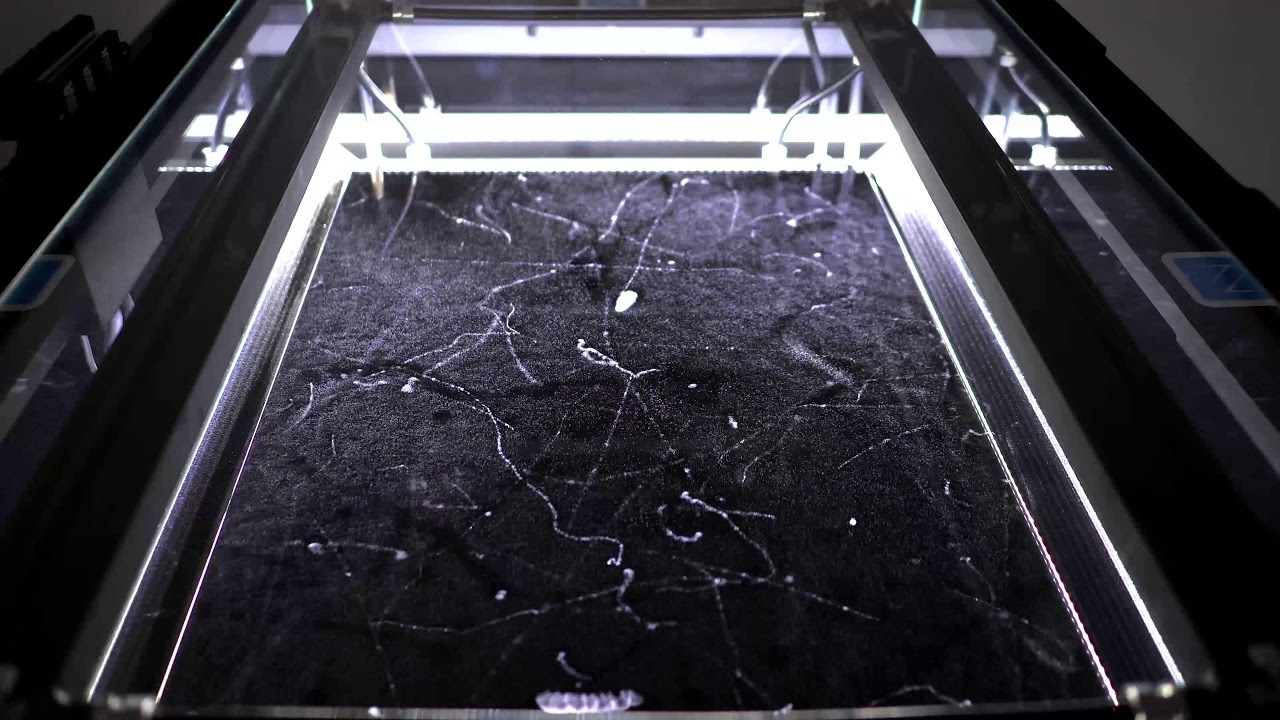
\includegraphics[width=0.9\textwidth]{Contents/cloudchamber.jpg}
    \caption{Illustration of the cloud chamber created by Wilson.
    Particles leave different tracks which help to identify them.}
    \label{fig:cloudchamber}
\end{figure}

Ionisation can be also detected via \emph{photographic emulsions}, in a very similar way as photos are captured. Usually a gelatin containing photo--sensible crystals (like $\text{AgB}_2$) is used: once exposed to light, these crystals can be detected using common photographic processing techniques. In the case of ionising particles, the track can be detected with high precision.

This kind of detection technique (which takes the name of \emph{nuclear emulsion}) has been developed by Powell in 1939 and has been used recently in neutrino experiments like Chorus and Opera.

The \emph{bubble chamber} was introduced in 1952 by Glaser and is based on the same principle as cloud chambers. In this case a super--heated liquid (brought under pressure at a temperature above its boiling point) is used. When a particle crosses the chamber, the pressure is decreased with a piston and the ionisation induces the formation of small bubbles, which can be photographed. The main improvement with respect to the Wilson's cloud chamber is the possibility of making these vessels very large to allow a precise three--dimensional reconstruction.

\begin{figure}
  \centering 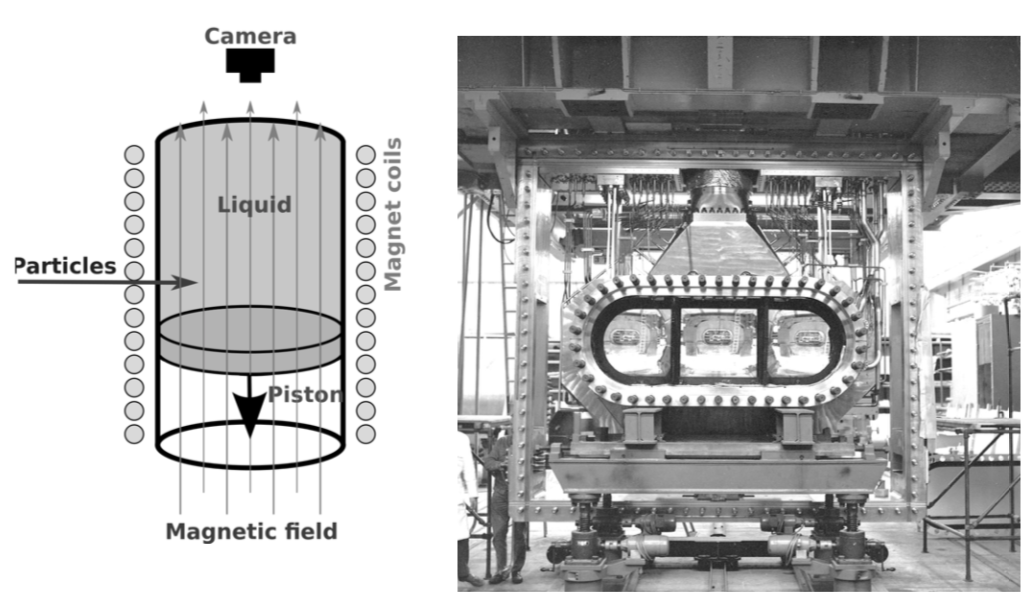
\includegraphics[width=0.9\textwidth]{detector6}
  \caption{Left: scheme of a bubble chamber. Right: $2\,\meter$ bubble chamber at CERN.}
  \label{fig:detector6}
\end{figure}

\subsection{Measurements on particle tracks}
Charged particle detectors allow to measure and identify particles; for example:
\begin{itemize}
\item the amount of ionisation that the particle leaves in the
  material gives information on its velocity $\beta c$;
\item some information on particle momentum can be extracted from multiple scattering.
\end{itemize}

Many additional information, and a precise measurement of momentum can
be extracted from a precise measurement of the particle track. In
particular, by having a charged particle travel through a region with a known magnetic field it is possible to extract
information on its charge and momentum from the curvature of
the particle track.

A particle with charge $q$ and mass $m$, which moves with velocity
$\vec{v}$ in a constant magnetic field $\vec{B}$ is affected by the
Lorentz force
\[\vec{F} = q\vec{v}\times\vec{B}\]
Let's study the motion of a particle in the plane orthogonal to
$\vec{B}$ (see figure \ref{fig:detector7}).

\begin{figure}
  \centering 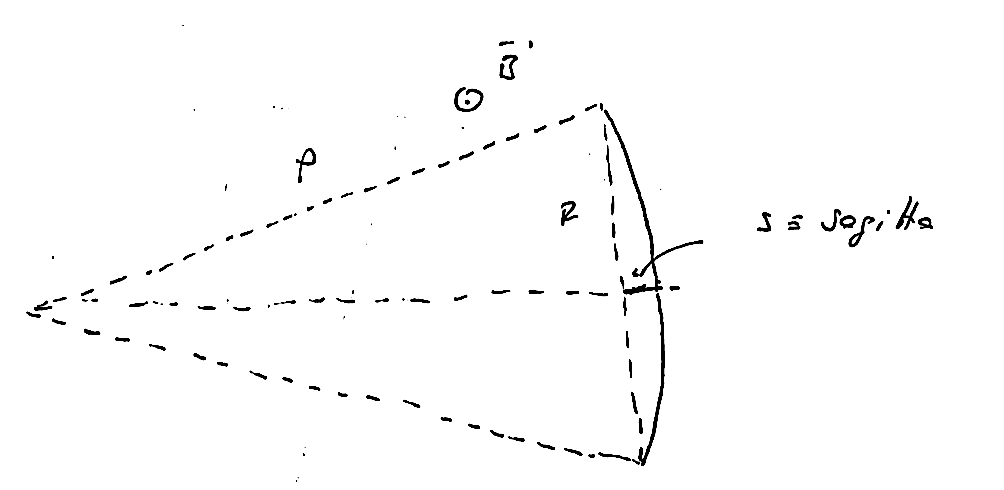
\includegraphics[width=0.6\textwidth]{detector7}
  \caption{Illustration of the geometry of a tracking detector immersed in a magnetic field. The particle curvature is described by the curvature radius $\rho$, which can be deduced for example from a measurement of the sagitta $s$.}
  \label{fig:detector7}
\end{figure}

We can write
\begin{eqnarray*}
  m\frac{v^2}{\rho}&=&qvb,\\
  mv &=& qB\rho
\end{eqnarray*}
which gives
\begin{equation}
  \label{eq:detector1}
  p = qB\rho.
\end{equation}
It is useful to express this equation in the following way (assuming $q = e$, using tesla and meters for $B$ and $\rho$, respectively):
\begin{equation}
  \label{eq:detector3}
  p\,\qq{\giga\electronvolt} = 0.3\,q\,\qq{C} \,B\,\qq{\tesla}\ \rho\,\qq{\meter}.
\end{equation}
This formula can be obtained by multiplying both
members of \ref{eq:detector1} by $c$ and using natural units.

Let's now consider again figure \ref{fig:detector7}, and assume that we measure the track of the particle in the region where the magnetic field acts. We can write
\begin{eqnarray*}
  \rho^2 &=& \rr{\frac{R}{2}}^2 + \rr{R-s}^2\\
         &=& \frac{R^2}{4} + \rho^2 + s^2 -2\rho s,\\
  s^2 -2\rho s &=& - \frac{R^2}{4},\\
\end{eqnarray*}
and in the limit of very small $s$ we can neglect the term proportional to $s^2$, and obtain
\[s = \frac{R^2}{8\rho}.\]
Using Eq. \eqref{eq:detector3} we get
\begin{equation}
  \label{eq:detector2}
  s = \frac{0.3\,B R^2}{8p},
\end{equation}
which finally gives:
\[p = \frac{0.3\,B R^2}{8s}.\]

It is clear that the accuracy on momentum measurement, assuming $B$ to be stationary and well known, depends on the measurement of $R$ and $s$. Considering only the uncertainty on $s$, the uncertainty on momentum $\Delta p$ can be written ads
\begin{eqnarray*}
  \Delta p &=& \frac{0.3\,BR^2}{8}\left|\dpar{\frac{1}{s}}{s}\right|\Delta s\\
          &=&\frac{0.3\,BR^2}{8s^2}\Delta s\\
           &=& \frac{0.3\,BR^2}{8}\rr{\frac{8p}{0.3\,BR^2}}^2 \Delta s\\
           &=& \frac{8p^2}{0.3\,BR^2}\Delta s,
\end{eqnarray*}
in which we used equation \ref{eq:detector2}. This can be written as
\[\frac{\Delta p }{p^2} = \frac{8}{0.3\,BR^2}\Delta s\]

Since the resolution on position measurement, and then on $s$ is constant, we get that:
\[\frac{\Delta p}{p} \propto p\]
This means that the resolution on the momentum measurement is directly proportional to the momentum itself.

Another typical case is the one of the magnetic analyser, shown in figure \ref{fig:detector8}. In this case, we measure the track of the particle before and after it gets deflected by a magnetic field.

\begin{figure}
  \centering 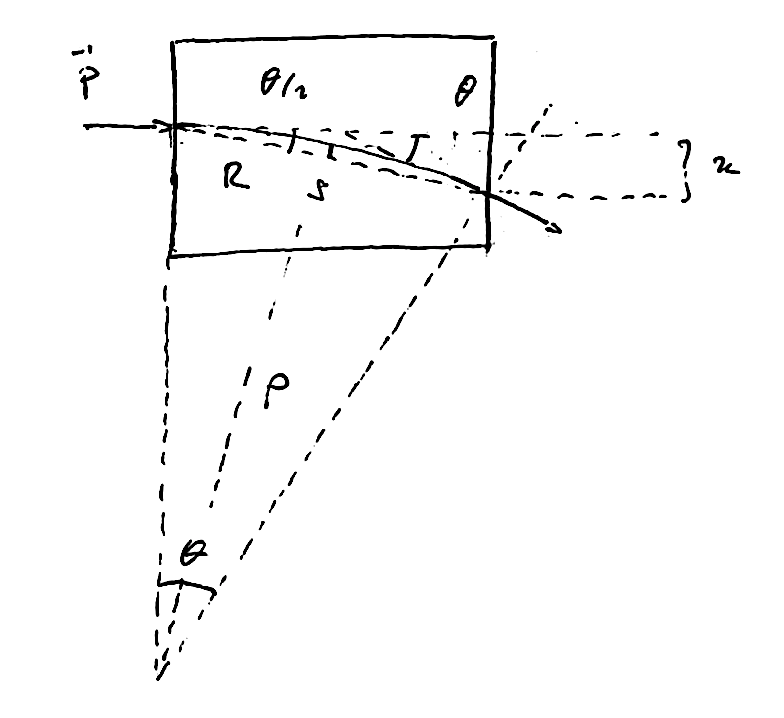
\includegraphics[width=0.6\textwidth]{detector8}
  \caption{Illustration of a magnetic analyser. We measure the track of the particle before and after the region where the magnetic field is present, i.e. we effectively measure the vertical displacement $x$ -- or, equivalently, the angle $\theta$ between the initial and final directions of the particle.}
  \label{fig:detector8}
\end{figure}

From the figure it's easy to get
\[\frac{\frac{R}{2}}{\rho} = \sin\frac{\theta}{2},\]
which for small angles becomes
\begin{eqnarray*}
  \frac{\frac{R}{2}}{\rho} &\sim& \frac{\theta}{2}\\
  R &\sim& \rho \theta,
\end{eqnarray*}
and using Eq. \eqref{eq:detector3}, in natural units, we have
\begin{eqnarray*}
  p &=& 0.3\, B\rho\\
    &=& 0.3\,B\frac{R}{\theta},\\
  p\theta &=& 0.3\,BR,
\end{eqnarray*}
i.e.
\[\theta = 0.3\,B\frac{R}{p}.\]
Since the displacement $x$ can be expressed as
\begin{eqnarray*}
  x &=& R\sin\frac{\theta}{2}\\
    &\simeq& R\frac{\theta}{2}  \\
  &=& \frac{0.3\,BR^2}{2p},
\end{eqnarray*}
i.e.
\[p = \frac{0.3\,BR^2}{2x},\]
as before we get
\[\Delta p = \frac{0.3\,BR^2}{2x^2}\Delta x,\]
and the resolution on $p$ is
\[\frac{\Delta p}{p^2} = \frac{2}{0.3\,BR^2}\Delta x.\]
Again, the resolution on momentum is proportional to the momentum itself since $\Delta x$ can be treated as a constant.


\subsubsection*{Key points}
\begin{itemize}
\item In order to reconstruct particle tracks, a strong magnetic field is required. High--momentum tracks need intense magnetic fields to be detectable.
\item There's a wide variety of detectors suitable for tracking (the one listed here are just few examples).
\item Some detectors can measure the velocity of the particle, or the ionisation released, or the transition radiation emitted.
\item The precision on the momentum measurement is strictly related to the precision on the position of the track points.
\item The choice of which kind of detector to use is strongly dependent on the volume which needs to be covered, the resolution or the rapidity of the emitted signal (some detectors with a very fast response are used as trigger).
\end{itemize}
%%%Local Variables:
%%% mode: latex
%%% TeX-master: "../book"
%%% End:
